% Options for packages loaded elsewhere
\PassOptionsToPackage{unicode}{hyperref}
\PassOptionsToPackage{hyphens}{url}
\PassOptionsToPackage{dvipsnames,svgnames,x11names}{xcolor}
%
\documentclass[
  12pt,
  a4paper,
  12pt]{article}

\usepackage{amsmath,amssymb}
\usepackage{setspace}
\usepackage{iftex}
\ifPDFTeX
  \usepackage[T1]{fontenc}
  \usepackage[utf8]{inputenc}
  \usepackage{textcomp} % provide euro and other symbols
\else % if luatex or xetex
  \usepackage{unicode-math}
  \defaultfontfeatures{Scale=MatchLowercase}
  \defaultfontfeatures[\rmfamily]{Ligatures=TeX,Scale=1}
\fi
\usepackage{lmodern}
\ifPDFTeX\else  
    % xetex/luatex font selection
  \setmainfont[]{Times New Roman}
\fi
% Use upquote if available, for straight quotes in verbatim environments
\IfFileExists{upquote.sty}{\usepackage{upquote}}{}
\IfFileExists{microtype.sty}{% use microtype if available
  \usepackage[]{microtype}
  \UseMicrotypeSet[protrusion]{basicmath} % disable protrusion for tt fonts
}{}
\usepackage{xcolor}
\setlength{\emergencystretch}{3em} % prevent overfull lines
\setcounter{secnumdepth}{5}
% Make \paragraph and \subparagraph free-standing
\ifx\paragraph\undefined\else
  \let\oldparagraph\paragraph
  \renewcommand{\paragraph}[1]{\oldparagraph{#1}\mbox{}}
\fi
\ifx\subparagraph\undefined\else
  \let\oldsubparagraph\subparagraph
  \renewcommand{\subparagraph}[1]{\oldsubparagraph{#1}\mbox{}}
\fi


\providecommand{\tightlist}{%
  \setlength{\itemsep}{0pt}\setlength{\parskip}{0pt}}\usepackage{longtable,booktabs,array}
\usepackage{calc} % for calculating minipage widths
% Correct order of tables after \paragraph or \subparagraph
\usepackage{etoolbox}
\makeatletter
\patchcmd\longtable{\par}{\if@noskipsec\mbox{}\fi\par}{}{}
\makeatother
% Allow footnotes in longtable head/foot
\IfFileExists{footnotehyper.sty}{\usepackage{footnotehyper}}{\usepackage{footnote}}
\makesavenoteenv{longtable}
\usepackage{graphicx}
\makeatletter
\def\maxwidth{\ifdim\Gin@nat@width>\linewidth\linewidth\else\Gin@nat@width\fi}
\def\maxheight{\ifdim\Gin@nat@height>\textheight\textheight\else\Gin@nat@height\fi}
\makeatother
% Scale images if necessary, so that they will not overflow the page
% margins by default, and it is still possible to overwrite the defaults
% using explicit options in \includegraphics[width, height, ...]{}
\setkeys{Gin}{width=\maxwidth,height=\maxheight,keepaspectratio}
% Set default figure placement to htbp
\makeatletter
\def\fps@figure{htbp}
\makeatother

\addtolength{\oddsidemargin}{-.5in}%
\addtolength{\evensidemargin}{-1in}%
\addtolength{\textwidth}{1in}%
\addtolength{\textheight}{1.7in}%
\addtolength{\topmargin}{-1in}%
\usepackage{booktabs}
\usepackage{longtable}
\usepackage{array}
\usepackage{multirow}
\usepackage{wrapfig}
\usepackage{float}
\usepackage{colortbl}
\usepackage{pdflscape}
\usepackage{tabu}
\usepackage{threeparttable}
\usepackage{threeparttablex}
\usepackage[normalem]{ulem}
\usepackage{makecell}
\usepackage{xcolor}
\usepackage{caption}
\makeatletter
\@ifpackageloaded{caption}{}{\usepackage{caption}}
\AtBeginDocument{%
\ifdefined\contentsname
  \renewcommand*\contentsname{Table of contents}
\else
  \newcommand\contentsname{Table of contents}
\fi
\ifdefined\listfigurename
  \renewcommand*\listfigurename{List of Figures}
\else
  \newcommand\listfigurename{List of Figures}
\fi
\ifdefined\listtablename
  \renewcommand*\listtablename{List of Tables}
\else
  \newcommand\listtablename{List of Tables}
\fi
\ifdefined\figurename
  \renewcommand*\figurename{Figure}
\else
  \newcommand\figurename{Figure}
\fi
\ifdefined\tablename
  \renewcommand*\tablename{Table}
\else
  \newcommand\tablename{Table}
\fi
}
\@ifpackageloaded{float}{}{\usepackage{float}}
\floatstyle{ruled}
\@ifundefined{c@chapter}{\newfloat{codelisting}{h}{lop}}{\newfloat{codelisting}{h}{lop}[chapter]}
\floatname{codelisting}{Listing}
\newcommand*\listoflistings{\listof{codelisting}{List of Listings}}
\makeatother
\makeatletter
\makeatother
\makeatletter
\@ifpackageloaded{caption}{}{\usepackage{caption}}
\@ifpackageloaded{subcaption}{}{\usepackage{subcaption}}
\makeatother
\ifLuaTeX
  \usepackage{selnolig}  % disable illegal ligatures
\fi
\usepackage[]{natbib}
\bibliographystyle{agsm}
\usepackage{bookmark}

\IfFileExists{xurl.sty}{\usepackage{xurl}}{} % add URL line breaks if available
\urlstyle{same} % disable monospaced font for URLs
\hypersetup{
  pdftitle={Political Leadership Survival in the Aftermath of Coups and Overstays: From Illegitimate Ascent to Unexpected Exit},
  pdfauthor={Zhu Qi},
  pdfkeywords={Political survival, Coups, Overstays},
  colorlinks=true,
  linkcolor={blue},
  filecolor={Maroon},
  citecolor={Blue},
  urlcolor={Blue},
  pdfcreator={LaTeX via pandoc}}


\begin{document}


\def\spacingset#1{\renewcommand{\baselinestretch}%
{#1}\small\normalsize} \spacingset{1}


%%%%%%%%%%%%%%%%%%%%%%%%%%%%%%%%%%%%%%%%%%%%%%%%%%%%%%%%%%%%%%%%%%%%%%%%%%%%%%

\date{February 12, 2024}
\title{\bf Political Leadership Survival in the Aftermath of Coups and
Overstays: From Illegitimate Ascent to Unexpected Exit}
\author{
Zhu Qi\\
}
\maketitle

\bigskip
\bigskip
\begin{abstract}
This paper delves into the duration of political leaders' tenures,
focusing on two specific categories: leaders who come into power through
coups and those who exceed their designated term limits. It argues that
the length of political leadership tenures is not solely determined by
their governing strategies but also by the means through which they
ascend to power. By employing a survival model, this study demonstrates
that leaders who surpass their term limits generally have longer tenures
compared to those entering through coups.
\end{abstract}

\noindent%
{\it Keywords:} Political survival, Coups, Overstays
\vfill

\newpage
\spacingset{1.9} % DON'T change the spacing!

\setstretch{1.75}
\section{Introduction}\label{introduction}

The investigation into the enduring tenure of certain leaders compared
to those with briefer terms has remained a focal point within the realm
of political science. This probing inquiry has garnered extensive
attention and undergone thorough analysis across numerous scholarly
works, as highlighted in Chapter 2.

Prior research examining the longevity of political leaders has
highlighted two prominent features. Firstly, scholars have primarily
concentrated on general frameworks that encompass either all regime
types or all autocracies, dedicating less attention to the exploration
of specific leader profiles. Secondly, existing studies have
predominantly revolved around analyzing the probability of irregular
leader exits using country-year data, leaving a void in discussions
regarding the duration of leadership tenures based on comprehensive
duration data.

Due to these significant gaps, this paper aims to conduct a comparative
analysis between two specific types of political leaders: those who rise
to power through coups and those who exceed their designated term
limits. Examining the tenures of these two irregularly ascended leaders
holds particular significance for two reasons.

Firstly, irregularly ascended leaders constitute the majority of
irregular exits from power. According to \citep{goemans2009}, between
1945 and 2015, among 1472 leaders who assumed office through regular
channels, around 213 exited irregularly (about 14.5\%). Conversely, out
of 308 leaders who assumed office through irregular means, roughly 158
(about 51.3\%) experienced irregular exits. Secondly, among irregularly
ascended leaders, the majority gained power through coups or overstays.
As per \citep{goemans2009}, out of 374 leaders who exited irregularly,
246 were ousted through coups, constituting 65.8\% of these cases.
Accordingly, there are 246 coup-entry leaders. Moreover, between 1945
and 2020, there were 106 attempts to overstay in power, of which 86 were
successful. This overstaying, detailed in ``Determinants of Incumbent
Overstay Attempts and Outcomes,'' can be perceived as a form of
self-coup, as incumbents orchestrate tactics to prolong their rule,
effectively staging coups against potential future leaders. Hence, it
becomes both relevant and enlightening to delve into and compare the
tenures of survival between coup-entry leaders and overstaying
(self-coup) leaders.

However, while existing research extensively delves into the factors
leading to coups or overstays, there remains a crucial need for more
attention directed towards what occurs after these irregular ascents.
Specifically, how do leaders' methods of entering power affect not only
their subsequent tenures but also their departures from power? This
study proposes that the manner in which leaders ascend to power
significantly impacts the duration of their leadership tenure. Unlike
leaders who overstay, those who enter through coups face more
substantial challenges concerning legitimacy, uncertainty, instability,
and power-sharing, potentially diminishing their survival duration.

\begin{figure}

\centering{

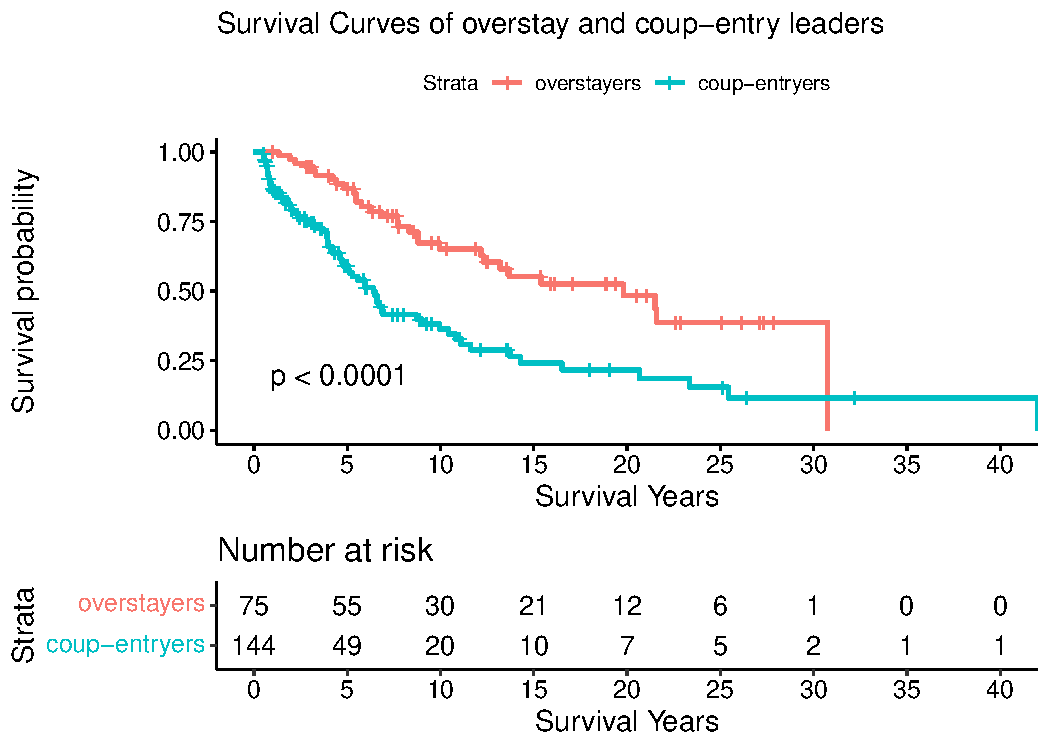
\includegraphics{survival_after_coups_jasa_files/figure-pdf/fig-logrank-1.pdf}

}

\caption{\label{fig-logrank}Kaplan-Meier plot for survival curves of
overstay and coup-entry leaders}

\end{figure}%

Utilizing a survival model, this paper suggests that leaders who surpass
their term limits generally enjoy longer tenures compared to those who
come into power through coups. Conducting a log-rank test in survival
analysis on the leaders dataset \citep{goemans2009} and the author's
incumbent overstay dataset reveals a distinct contrast: overstay leaders
demonstrate notably extended survival rates in comparison to coup-entry
leaders. Specifically, according to Figure~\ref{fig-logrank}, the
average survival time post-overstay, excluding their original term
duration, is approximately 10.8 years. In contrast, leaders who gain
power via coups tend to have an average survival time of 5.3 years,
representing an average shortfall of 5 years in their tenure
\footnote{The data excluded leaders who survived less than 180 days.}.

This study could offer dual contributions. First, it emphasizes that the
duration of survival and unexpected exits is not solely dictated by
leaders' conduct after assuming power but is fundamentally shaped by
their methods of gaining power. It accentuates a significant difference
in tenures between overstaying leaders and coup-entry leaders. Second,
it provides empirical measurements to compare the tenure duration of
these two irregularly ascended leaders, offering insights into their
distinct impacts on the longevity of leadership.

After the introduction, the second section encompasses a comprehensive
literature review on political survival and highlighting the
contributions of this paper might offer. The third chapter delves into
the examination of factors influencing the survival of leaders who have
ascended to power through unconstitutional means. Chapter 4 provides an
account of the methodology and data employed, utilizing a survival model
for a comprehensive analysis of the determinants of leaders' survival.
Chapter 5 presents the findings of this analysis, facilitating an
in-depth discussion of the results. Finally, in Chapter 6, the paper
concludes by synthesizing these findings and exploring their broader
implications.

\newpage

\section{Literature review: The dynamics of leadership survival in
different
scenarios}\label{literature-review-the-dynamics-of-leadership-survival-in-different-scenarios}

In their seminal work, \citet{buenodemesquita2003} conducted a
comprehensive examination of leaders spanning diverse political
landscapes, encompassing democracies and autocracies, as well as
parliamentary and presidential systems, while accounting for both
civilian and military contexts. Their aim was to provide an general
explanation for the dynamics of political leadership survival within a
universal framework. Proposing a universal theoretical framework
regarding the political survival is highly intriguing. However, it is
crucial to acknowledge the challenges that must be addressed in order to
provide a more general theory of leadership survival across all types of
regimes.

First of all, the rules governing power transitions differ drastically
between democracies and autocracies. In most autocratic regimes, the
process of leadership selection remains shrouded in secrecy. Expressing
dissenting views, whether as potential challengers or supporters of
challengers, can be perilous. In Russia, despite the presence of general
elections, challengers frequently face severe consequences such as
assassination, poisoning, imprisonment, or exile. Due to the lack of
transparent and fair conventional procedures for power transitions, it's
challenging to assess who holds more power or has more supporters. A
dictator could potentially survive a lengthy tenure despite weak support
because the true balance of power remains undisclosed. Conversely, a
powerful ruler could be ousted by a small number of guards because the
army or other supporters hesitate to fight for them due to a lack of
information regarding their predominant status in the power balance.
Thus, accurately calculating selectorates or coalitions, as
\citet{buenodemesquita2003} did in their research, becomes impossible in
such scenarios. In contrast, in democracies, challengers can openly vie
for leadership without fear. Their support rates are easily discernible,
and they can seek to gain more supporters through public speeches, TV or
newspaper advertisements, or assemblies. If their support rates are not
adequate to challenge the incumbents, different groups can try to
collaborate, facilitating power transitions with a slightly higher level
of support.

Secondly, the division of residents into different coalitions or groups
may not hold as much relevance in democracies when compared to
autocracies. In democratic systems, while those who support and vote for
incumbents may witness their advocated policies enacted, those opposing
them still experience the same policies. For instance, if a candidate
advocating for lower taxes wins an election, it doesn't lead to lower
taxes for the elected leaders' supporters and higher taxes for their
opponents; both groups encounter identical tax levels. This dynamic
differs significantly in autocratic regimes, where distinct groups
benefit unequally based on their status and relationships with the
rulers.

Furthermore, our interest in analyzing political survival stems from
irregular and unforeseen power transitions. Discussing regular and
expected leadership tenures is neither necessary nor pertinent in this
context. As previously mentioned, over 85\% of leaders entering power
through regular means also exited in a regular manner
\citep{goemans2009}. Many political leaders, especially in democracies
and some autocracies, experience predictable and routine tenures.
Consider the case of the United States, where presidents can serve up to
eight years if re-elected for a second term, or at least complete a full
four-year term despite underperformance. Similarly, in autocratic Mexico
from 1919 to 2000, each president served a fixed six-year term without
facing overthrows or overstays, as noted by \citep{klesner2019}.
Analyzing the survival of such leaders might seem futile as their power
transitions typically occur within the bounds of constitutional rules.

On the other hand, leaders who come into power through irregular means
paint a more intricate and unpredictable picture. Take, for instance,
Henri Namphy, who assumed the presidency of Haiti following a coup in
June 1988, only to be ousted by another coup a mere three months later
in September of the same year. However, Qaddafi, the dictator of Libya,
seized power in a coup in 1969 and ruled for over 40 years before being
killed in 2011 by NATO-backed rebel forces \citep{goemans2009}. Certain
dictators maintain an indefinite grip on power until their death,
subsequently transferring authority to family members, such as sons in
the cases of Syria and North Korea or brothers in the context of Cuba.

Given the distinct nature of political leadership survival in various
regimes, scholars have increasingly focused on understanding the
survival dynamics specific to certain regime types, such as democracies
\citep{svolik2014} and autocracies \citep{davenport2021}. Notably,
considerable academic attention has been drawn towards unexpected
tenures, particularly those leaders who either fail to complete their
original terms or overstay their terms. Scholars have predominantly
revolved around two primary dimensions. The first dimension encompasses
contextual conditions and resources available to leaders. These factors
include elements such as the leaders' personal competence
\citep{yu2016}, societal stability \citep{arriola2009}, economic
development level \citep{palmer1999, williams2011}, access to natural
resources \citep{smith2004, quirozflores2012}, and external support
networks \citep{licht2009, wright2008, thyne2017}. The second dimension
delves into the strategies implemented by leaders in enacting their
political and economic policies. This includes their responses to
challengers and dissent within their regimes
\citep{escribà-folch2013, davenport2021}, as well as strategies used in
policy-making \citep{gandhi2007, morrison2009}.

Unsurprisingly, a considerable focus in previous studies has been
directed towards coups, given their status as a prominent pathway
leading to the exit of authoritarian leaders
\citep{svolik2008, frantz2016}. Literature on leadership survival has
examined strategies aimed at preventing coups
\citep{powell2017, sudduth2017, debruin2020}, as well as analyses of how
leaders extend their tenures post-surviving failed coup attempts
\citep{easton2018}. For instance, \citet{sudduth2017a}, while primarily
focused on purge strategies, examines the post-coup actions of a
dictator. The central argument suggests that leaders ascending through
coups experience a temporary surge in influence compared to elites
immediately following the coups, making them less prone to subsequent
ousting by coup attempts. This argument challenges the traditional
notion that new leaders are generally in a weak position at the start of
their tenure \citep{roessler2011}. Despite this distinction, both
Sudduth and prior scholars concur that new leaders tend to purge rival
elite groups to consolidate their power. Sudduth argues that dictators
undertake purges when they can do so without significant risk, while
traditional views suggest purges occur when dictators perceive imminent
threats. However, it's imperative to acknowledge that new leaders,
particularly those ascending through unconventional means, don't adhere
to a universal pattern of inherent weakness or strength. Leadership
transitions unfold in varied contexts, presenting leaders with diverse
challenges.

Scholars have extensively analyzed the endurance of political leaders
across various spheres, examining universal frameworks, autocratic
regimes, and the aftermath of failed challenges, including coup
attempts. However, there remains a notable gap in discussions
surrounding the survival dynamics of leaders who consolidate power after
successful coups or prolonged incumbency. Specifically, there has been
limited exploration and comparison of the survival tenures between
overstay leaders and coup-entry leaders. This study seeks to address
this gap by scrutinizing and outlining the duration of survival among
these two distinct categories of leaders.

\newpage

\section{Political survival dynamics of overstay and coup-entry
leaders}\label{political-survival-dynamics-of-overstay-and-coup-entry-leaders}

In this paper, I maintain the definition of ``overstay'' as delineated
in my earlier paper, ``Determinants of Incumbent Overstay Attempts and
Outcomes'', referring to situations where incumbent political leaders
strive to exceed the maximum time permitted by constitutional norms or
unwritten customs. A successful overstay is determined by an extension
of power lasting at least six months or longer.

Regarding the definition of a ``coup'', I will adopt the definition
outlined by Powell and Thyne: coups are characterized as ``illegal and
overt attempts by the military or other elites within the state
apparatus to unseat the sitting executive'' \citep[p252]{powell2011}.
They categorize a coup attempt as successful if the perpetrators seize
and retain power for a minimum of seven days. To align with the
successful overstays discussed in this paper, I will focus on instances
where the usurpation of power endures for at least six months.

Engaging in discussions on the survival strategies employed by political
leaders in non-democratic systems presents a considerable challenge.
This challenge is rooted in the intricate nature of power transitions
within autocratic regimes, which lack a consistent and universally
applicable pattern or set of conventions. In specific instances, such as
Middle Eastern monarchies, the transfer of power doesn't strictly adhere
to a hereditary father-to-son lineage, further complicating the
landscape. Moreover, even if there are established rules governing power
transitions, they are often flouted by incumbents or coup leaders.

Nevertheless, amidst the diversity in regime types and leadership
styles, leaders who prolong their rule through self-coups and those who
seize power through coups exhibit certain similarities. Understanding
these shared tactics provides insight into their strategies for
survival.

The first aspect concerns the issue of legitimacy. Leaders who ascend
through coups lack legitimacy as they seize power through force or other
unconventional means. While many leaders prolong their tenures through a
façade of constitutional procedures, such as judgments by the Supreme
Court, congressional votes, or even referendums, they often manipulate
these processes to maintain control. It's commonly understood by ruling
elites, opposition parties, and the populace that these leaders lack
legitimacy. This lack of legitimacy can sometimes justify the cause of
those seeking their replacement, even if the means used are
unconstitutional.

The second characteristic revolves around the uncertainty surrounding
power transitions. This uncertainty creates ambiguity not only for
ruling elites and ordinary citizens but also for the leaders themselves
regarding when, how, and to whom power might be transferred. Such
uncertainty breeds inherent instability. Amidst such instability, people
experience a lack of security. This perception often leads to the belief
that the current ruler is incompetent and should be replaced by someone
more powerful or capable. Consequently, the ruling elite or opposition
factions may exploit the instability as an opportunity to challenge
existing power structures.

The third aspect revolves around the equilibrium of power. In
autocracies, governance typically rests with a minority faction that
possesses a highly structured organization, distinctly contrasting with
the decentralized and disorganized subjects. Even amid protests or
uprisings, ruling groups adeptly suppress such incidents individually.
The possibility of overthrowing tyranny arises if the subjects can
coalesce their efforts. However, the principal obstacle lies in the
formidable challenge of surmounting the collective action problem.
Autocratic dictators commonly adopt a ruling strategy focused on
preventing unity among subjects and complicating endeavors to address
collective action issues. This elucidates why dictatorships curtail free
expression, assembly, and association. The absence of free public
expression and association renders the power balance unclear.
Consequently, rulers maintain relative power advantages over not only
the elites but also the subjects.

The convergence of illegitimacy, uncertainty, and power equilibrium, as
highlighted in Table~\ref{tbl-aspects}, significantly influences the
lifespan of a regime. However, when juxtaposed with leaders who seize
power through coups, those who overextend their terms enjoy a relatively
favorable position across these three facets.

\begin{longtable}[]{@{}
  >{\raggedright\arraybackslash}p{(\columnwidth - 4\tabcolsep) * \real{0.2083}}
  >{\raggedright\arraybackslash}p{(\columnwidth - 4\tabcolsep) * \real{0.3194}}
  >{\raggedright\arraybackslash}p{(\columnwidth - 4\tabcolsep) * \real{0.4722}}@{}}
\caption{Key Distinctions in Survival Tenures: Overstay versus
Coup-Entry Leaders}\label{tbl-aspects}\tabularnewline
\toprule\noalign{}
\begin{minipage}[b]{\linewidth}\raggedright
\textbf{Aspect}
\end{minipage} & \begin{minipage}[b]{\linewidth}\raggedright
\textbf{Overstay Leaders}
\end{minipage} & \begin{minipage}[b]{\linewidth}\raggedright
\textbf{Coup-Entry Leaders}
\end{minipage} \\
\midrule\noalign{}
\endfirsthead
\toprule\noalign{}
\begin{minipage}[b]{\linewidth}\raggedright
\textbf{Aspect}
\end{minipage} & \begin{minipage}[b]{\linewidth}\raggedright
\textbf{Overstay Leaders}
\end{minipage} & \begin{minipage}[b]{\linewidth}\raggedright
\textbf{Coup-Entry Leaders}
\end{minipage} \\
\midrule\noalign{}
\endhead
\bottomrule\noalign{}
\endlastfoot
Legitimacy & Normally attained through lawful procedures, but lacking
recognized legitimacy. & Attained unlawfully, devoid of legitimacy. \\
Uncertainty in Power Transitions & Initially stable; uncertainty grows
with prolonged tenure, especially without designated successors as
leaders age. & Significant uncertainty initially; stability emerges as
power is consolidated, yet prolonged leadership poses similar challenges
as overstay, fostering instability. \\
Power Sharing & Fewer challenges in power equilibrium due to successful
overstay. & Confront power-sharing issues promised during coup staging,
potentially triggering dissatisfaction among supporters if agreements
are unmet. \\
\end{longtable}

\subsection{Legitimacy}\label{legitimacy}

The core of a coup inherently lacks legitimacy, being deemed ``illegal''
due to its sudden and unconstitutional nature. Successful coups serve as
a catalyst, publicly spotlighting alternate, non-constitutional paths to
seize power. This visibility inadvertently encourages imitation,
especially among those less inclined to ascend to power through lawful
channels, leading to a surge in illegitimate power seizures. Henri
Namphy's leadership during Haiti's 1988 coup serves as an typical
example, swiftly followed by his own removal through another coup.
Haiti's history records instances of multiple coups within a single
year---such as 3 in 1957, and 2 each in 1988, 1989, and 1991---a
narrative echoed in numerous other coup-prone nations. Notable examples
post-2000 include 2 coups in 2001 in Burundi, 2 in 2021 in Sudan, and 2
in 2022 in Burkina Faso \citep{powell2011}. As reflected in
Table~\ref{tbl-coups}, 15 countries have weathered at least 10 coups
since 1950, with most exceeding 5 successful attempts
\citep{powell2011}. These 15 nations collectively accounted for 40\% of
total coup attempts and 38\% of successful coups. In these frequent-coup
countries, coups have even surpassed constitutionally guided power
transitions in frequency. Both ruling groups and the populace have grown
accustomed to coups, perceiving them as an acceptable means of power
transition. Recent occurrences in Burkina Faso (2022) and Niger (2023)
demonstrate this familiarity, where some individuals treated these
events more akin to festive celebrations rather than coups.

Moreover, coups not only breed subsequent coups but also embolden
external challengers, fostering uprisings, revolutions, and civil wars,
as highlighted by \citet{dahl2023}.

\begin{table}

\caption{\label{tbl-coups}Frequency of Coups by Country (1950--2023)}

\centering{

\centering
\begin{tabular}{>{\raggedright\arraybackslash}p{4.5cm}>{\centering\arraybackslash}p{4.5cm}>{\centering\arraybackslash}p{4.5cm}}
\toprule
\textbf{Country} & \textbf{Coup attempts} & \textbf{Successful coups}\\
\midrule
\cellcolor{gray!10}{Bolivia} & \cellcolor{gray!10}{23} & \cellcolor{gray!10}{11}\\
\addlinespace
Argentina & 20 & 7\\
\addlinespace
\cellcolor{gray!10}{Sudan} & \cellcolor{gray!10}{17} & \cellcolor{gray!10}{6}\\
\addlinespace
Haiti & 13 & 9\\
\addlinespace
\cellcolor{gray!10}{Venezuela} & \cellcolor{gray!10}{13} & \cellcolor{gray!10}{0}\\
\addlinespace
Iraq & 12 & 4\\
\addlinespace
\cellcolor{gray!10}{Syria} & \cellcolor{gray!10}{12} & \cellcolor{gray!10}{8}\\
\addlinespace
Thailand & 12 & 8\\
\addlinespace
\cellcolor{gray!10}{Ecuador} & \cellcolor{gray!10}{11} & \cellcolor{gray!10}{5}\\
\addlinespace
Burundi & 11 & 5\\
\addlinespace
\cellcolor{gray!10}{Guatemala} & \cellcolor{gray!10}{10} & \cellcolor{gray!10}{5}\\
\addlinespace
Honduras & 10 & 6\\
\addlinespace
\cellcolor{gray!10}{Burkina Faso} & \cellcolor{gray!10}{10} & \cellcolor{gray!10}{9}\\
\addlinespace
Sierra Leone & 10 & 5\\
\addlinespace
\cellcolor{gray!10}{Ghana} & \cellcolor{gray!10}{10} & \cellcolor{gray!10}{5}\\
\bottomrule
\end{tabular}

}

\end{table}%

For leaders surpassing their designated terms, the situation diverges.
As incumbents, they abuse their power to manipulate the power transition
dynamics. They might reinterpret or amend the constitution, utilizing
avenues like parliamentary votes, supreme court decisions, or
referendums, with aspirations for prolonged or even lifelong tenure. Yet
fundamentally, most instances of overstaying lack authentic legitimacy
as such leaders often exploit their authority, resorting at times to
illegal measures like arresting, expelling, or even assassinating
opposition figures\footnote{\url{https://www.france24.com/en/live-news/20221123-vladimir-putin-s-critics-dead-jailed-exiled}:
  Vladimir Putin's critics: dead, jailed, exiled. Accessed on Dec 23,
  2023.}. Consequently, these alterations in leadership tenure and power
transitions do not genuinely reflect the populace's will. Nonetheless,
it's notable that, on the surface, the methods employed by overstay
leaders carry a semblance of legitimacy compared to coups. Even if
contesting their legitimacy, challengers are normally constrained to
adopt lawful means.

Additionally, overstaying might attract imitators, yet replicating
overstaying differs significantly from replicating coups. While coups
can happen at any moment, overstaying requires a prerequisite---those
seeking to overstay must initially occupy leadership positions. Even if
challengers openly reject legitimacy and attempt to employ similarly
illegitimate methods, such as orchestrating coups to oust overstay
leaders, it presents a far greater challenge, as it demands considerable
strength or substantial support. Conversely, an overstay leader
inherently possesses a position of advantage in terms of power. For
instance, in 2018, China's National People's Congress sanctioned the
removal of the two-term limit on the presidency---only two delegates
opposed the change, and three abstained out of 2,964 votes---effectively
granting Xi Jinping the potential to remain in power for
life\footnote{\url{https://www.bbc.co.uk/news/world-asia-china-43361276}:
  China's Xi allowed to remain `president for life' as term limits
  removed. Accessed on Dec 23, 2023.}. Similarly, in Russia's 2020
constitutional referendum, 79\% of valid votes supported changes to the
constitution enabling Putin to potentially rule until 2036\footnote{\url{https://www.ucl.ac.uk/news/2020/jul/analysis-vladimir-putin-secures-constitutional-changes-allowing-him-rule-until-2036}:
  Analysis: Vladimir Putin secures constitutional changes allowing him
  to rule until 2036. Accessed on Dec 23, 2023.} . While these figures
may not accurately reflect genuine support from ruling groups or the
populace, they do underscore the consolidation of power by the
incumbents .

Hence, from the legitimacy standpoint, while both overstaying leaders
and coup-entry leaders lack genuine legitimacy, the former retain an
edge in superficial legitimacy and are more powerful, potentially
leading to longer-lasting regimes than those initiated by coup-entry
leaders.

\subsection{Uncertainty}\label{uncertainty}

As discussed earlier, both leaders who overstay their terms and those
who come to power through coups contribute to uncertainty within their
regimes. However, regimes led by overstay rulers generally exhibit
comparatively lower levels of overall uncertainty.

In the aftermath of coups, uncertainty arises concerning the identity of
the leader and the duration of their tenure. The majority of coup
leaders have retained power since their coups, such as Gamal Abdel
Nasser in Egypt since the 1954 coup, Muammar Gaddafi in Libya following
the 1969 coup, and Idi Amin in Uganda after the 1971 coup
\citep{geddes2018}. Some coup leaders have claimed to intend to transfer
power to constitutionally elected leaders but failed to honor their
commitments, as seen in the case of the military junta in Myanmar after
the 2021 coup. Despite promising a new election after a year-long state
of emergency, the military junta extended the emergency multiple times
and retained power until the end of 2023\footnote{\url{https://thediplomat.com/2023/08/myanmar-junta-extends-state-of-emergency-for-fourth-time/}:
  Myanmar Junta Extends State of Emergency for Fourth Time. Accessed on
  Dec 24, 2023.}. Moreover, within military juntas themselves,
uncertainties persist. For instance, following the Chilean Coup in 1973,
a military junta initially planned to rotate the presidency among the
commanders-in-chief of the four military branches. However, General
Pinochet consolidated his control and retained power in Chile until 1990
\citep{svolik2012}.

Notably, some coup leaders have honored their promises and restored
power to constitutional civilian governments. For instance, after the
2010 coup in Niger, a new constitution reinstated civilian rule and
implemented a strict two-term limit on the presidency within the same
year \citep{ginsburg2019}.

In contrast, situations involving overstaying leaders offer more
straightforward answers regarding who will rule and for how long.
Overstayed incumbents remain in power for extended periods, often aiming
to prolong their tenures as much as possible. For instance, leaders like
Putin in Russia and Xi Jinping in China are less inclined to voluntarily
relinquish power unless forcibly removed. Even in cases like President
Menem of Argentina, who successfully overstayed his term until 1993 but
failed in his attempt for another term in 1999, his extended tenure
still lasted for a full five-year term \citep{llanos2019}.

Moreover, uncertainties not only revolve around who leads and for how
long but also concerning the leadership style and governance approach.
Coup-entry leaders face the need to restructure top officials and
substantiate their actions by implementing substantial changes after
toppling incumbents. In contrast, overstaying leaders encounter fewer
obstacles, as their regimes experience fewer abrupt changes. They are
less pressured to dismantle the existing ruling paradigm and establish a
new order.

Hence, comparatively, the rule of overstaying leaders tends to be less
uncertain than that of coup-entry leaders, aiding overstaying leaders in
stabilizing their governance and increasing their likelihood of enduring
longer than coup-entry leaders.

\subsection{Equilibrium of power}\label{equilibrium-of-power}

Autocratic rulers often grapple with a predicament known as the
``Guardianship dilemma'' in maintaining their authority. They find
themselves in need of loyal subordinates while also requiring competent
followers to manage intricate challenges and suppress opposition.
However, these capable supporters might eventually pose a threat to
their rule \citep{wintrobe2012, mcmahon2015, geddes2018}. More often
than not, heightened competence coincides with increased ambition.
Hence, the art of establishing and preserving a delicate power balance
becomes an intricate skill. Comparatively, leaders who come to power
through coups face even more daunting challenges in navigating the
perilous game of power equilibrium. They must establish a stable power
equilibrium initially, whereas entrenched leaders only need to maintain
an existing balance. Nonetheless, restoring a disrupted balance of power
is significantly more challenging than sustaining an already established
equilibrium.

Leaders who seize power through coups inevitably disrupt the existing
balance of power, necessitating the establishment of a new equilibrium,
even in seemingly peaceful scenarios. The removal of previous rulers
mandates the dismantling of the established governing structure and a
reshuffling of high-ranking officers and officials. These actions
inherently sow unrest and create adversaries for the new leadership,
making the restoration of order and the establishment of a balanced
power structure notably challenging. In order to establish consolidate
power, coup-leaders often have to comprise to internal or external power
challengers. However, more often than not, these comprises are not
stable and easy to break. For instance, consider Jean-Bertrand Aristide,
the president of Haiti, who was ousted in a 1991 coup and forced into
exile. Despite this, his supporters retained significant political
influence, ultimately facilitating Aristide's return to power in 1994
\citep{bermeo2016}.

Navigating internal power dynamics among coup leaders presents
significant challenges. For instance, after the Chilean coup in 1973, a
fleeting balance prevailed among the four branches of the military
junta. However, this fragile equilibrium was short-lived as Pinochet
consolidated absolute power in 1974 \citep{geddes2018}. However, taking
an uncompromising stance within the leadership does not always proceed
seamlessly, as seen in Pinochet's case. Such actions may provoke
backlash even from close allies. In Uganda, President Obote's attempt to
undermine the army commander-in-chief, Idi Amin, resulted in Amin
garnering the support of the majority of the army and ultimately ousting
Obote in a military coup in 1971. Similarly, in Pakistan in 1999,
shortly after Prime Minister Sharif dismissed powerful army chief
General Pervez Musharraf, Sharif himself was ousted in a coup
orchestrated by Musharraf and his military supporters
\citep{sudduth2017}. The situation becomes even more intricate when
there is a risk of civil war. According to \citet{roessler2011}, leaders
may endeavor to diminish the probability of subsequent coups,
potentially increasing the likelihood of societal rebellions and civil
wars.

The combination of these factors contributes to a shorter expected
lifespan of coup-entry leaders \citep{dahl2023} compared to the
relatively longer tenures of overstaying leaders. As previously
mentioned, the average survival period following an overstay is
approximately five years longer than that of leaders entering power
through coups (Figure~\ref{fig-logrank}). Building upon these
observations, I would like to propose the following hypothesis:

\textbf{Hypothesis:} Political leaders who successfully prolong their
tenure in power are more likely to experience extended regime survival
compared to leaders who come to power through coups.

In the subsequent section, I will outline the research methodology
utilized in this paper. I intend to introduce several control variables
to determine if the hypothesis remains persistent and robust.

\newpage

\section{Data and method}\label{data-and-method}

\subsection{Data}\label{data}

The main variables are as follows.

\subsubsection{Dependent variables}\label{dependent-variables}

\begin{itemize}
\item
  \textbf{Survival time:} the duration of leaders' tenure in days. For
  coup-entry leaders, this time span initiates on the day they assume
  power, while overstaying leaders' tenure begins on the expiration date
  of their initial term. For instance, considering Xi Jinping's case, he
  assumed power in 2013, successfully removing term limits in 2018.
  However, his initial two-term tenure was due to end in 2023. Hence,
  his survival time commences from 2023 rather than 2013, signifying the
  start of his original tenure. The survival time concludes on the day
  the leader exits office, applying to both coup-entry and overstaying
  leaders.
\item
  \textbf{End point status:} 0 = censored, 1 = ousted. I categorized
  ousting by force as 1, even in cases where some leaders
  ``voluntarily'' resigned under pressure. Other methods of leaving
  office are considered censored, which can encompass situations where
  leaders appoint their successors, opt for democratic means of
  overturn, face health-related issues, or encounter natural death.
\end{itemize}

\subsubsection{Independent variable}\label{independent-variable}

\begin{itemize}
\tightlist
\item
  \textbf{Leader type:} Group A = overstaying leader, Group B =
  coup-entry leader. This variable is the primary independent variable
  of interest, as it serves as the basis for comparison of survival time
  between the two types of leaders.
\end{itemize}

The dependent and independent data are sourced from the author's
incumbent overstay dataset and the leaders dataset by
\citep{goemans2009}.

\subsubsection{Control variables}\label{control-variables}

\begin{itemize}
\item
  \textbf{Indicators of Economic Influence:} To evaluate economic
  influence, I rely on two primary indicators: the trend in GDP growth
  (\texttt{GDP\_growth\_trend}) and the logarithm of GDP per capita
  (\texttt{GDP\_pc\_log)}. The GDP\_growth\_trend is determined by
  contrasting the GDP growth in the year of a coup entry or overstaying
  with the preceding 3-year moving average of the growth rate. The
  dataset employed for these metrics is sourced from V-Dem Data.
\item
  \textbf{Degree of Democracy:} The level of democracy is gauged using
  Polity 5 scores (\texttt{polity}) at the entry year for each
  respective country. This dataset is sourced from the Center for
  Systemic Peace (CSP)\footnote{Center for Systemic Peace:
    \url{https://www.systemicpeace.org}. Accessed on Dec 24, 2023.}.
\item
  \textbf{Population Size:} Accounting for its potential impact on
  leaders' tenures, the log population size (\texttt{pop\_log}) is
  considered. This data is obtained from the V-Dem Data and is evaluated
  in relation to its influence on leadership survival.
\item
  \textbf{Political Stability:} The stability of the political landscape
  is crucial in evaluating the survival tenures of leaders. To quantify
  this aspect, the Major Episodes of Political Violence Variables
  dataset from the CSP is utilized to measure political stability
  (\texttt{polstab}) at the leader's entry year.
\item
  \textbf{Leader's Age:} The age of the leader at the entry year serves
  as an additional variable in the analysis, providing insight into
  potential correlations with leadership survival. This data is sourced
  from the leaders dataset by \citep{goemans2009}.
\end{itemize}

\subsection{Method}\label{method}

In order to test the hypothesis, I will employ two cox models to analyze
the survival tenures of leaders who overstay their terms and those who
come to power through coups. The first model will utilize the Cox
proportional hazards model (referred to as the Cox PH model), where I
only use the variables at the entry year and do not consider the changes
of these variables among leaders' survival times.

However, except the main concern variable in this research, the leader
type, the control variables, such as economic performance, Polity5,
political stability, do change over time. The second model will take
this into consideration and use the time-dependent Cox model (referred
to as the Time-dependent Cox model).

Unlike the Kaplan-Meier model, the Cox model enables the estimation of
the impacts of multiple factors. Although it does not directly estimate
the duration of tenure in office, it evaluates the hazard rate
associated with being ousted from power, which essentially represents
different facets of the same phenomenon. As a leader's cumulative hazard
of being ousted increases, their probability of survival in office
decreases.

\begin{equation}
\begin{aligned}
Surv(survival\_time, status) &= group + \\
&GDP\_growth\_trend + GDP\_pc\_log + \\
&pop\_log + polity5 + polstab + age
\end{aligned}
\end{equation}

\newpage

\section{Outcome and discussion}\label{outcome-and-discussion}

Building on the preceding discussion, I investigated my hypothesis
regarding the likelihood of prolonged regime survival among leaders who
overstay their terms compared to those who assume power through coups.
The regression results of both the Cox PH model and the Time-dependent
Cox model are presented in Table~\ref{tbl-cox}.

\setlength{\LTpost}{0mm}

\begin{longtable}{lcccccccc}

\caption{\label{tbl-cox}Cox models for survival time of different types
of leaders}

\tabularnewline

\toprule
 & \multicolumn{4}{c}{\textbf{Cox PH Model}} & \multicolumn{4}{c}{\textbf{Time-dependent Cox Model}} \\ 
\cmidrule(lr){2-5} \cmidrule(lr){6-9}
\textbf{Characteristic} & \textbf{N} & \textbf{Event N} & \textbf{HR}\textsuperscript{\textit{1,2}} & \textbf{SE}\textsuperscript{\textit{2}} & \textbf{N} & \textbf{Event N} & \textbf{HR}\textsuperscript{\textit{1,2}} & \textbf{SE}\textsuperscript{\textit{2}} \\ 
\midrule\addlinespace[2.5pt]
\textbf{Coup-entry leaders} &  &  &  &  &  &  &  &  \\ 
    Overstay leaders & 75 & 30 & 1.00 & — & 739 & 28 & 1.00 & — \\ 
    Coup-entry leaders & 144 & 73 & 2.49*** & 0.251 & 796 & 73 & 2.41*** & 0.257 \\ 
\textbf{GDP Growth Trend} & 219 & 103 & 1.00 & 0.001 & 1,535 & 101 & 1.00 & 0.005 \\ 
\textbf{GDP per capita: log} & 219 & 103 & 0.73* & 0.126 & 1,535 & 101 & 0.73** & 0.121 \\ 
\textbf{Population: log} & 219 & 103 & 1.25 & 0.139 & 1,535 & 101 & 1.19 & 0.134 \\ 
\textbf{Polity5} & 219 & 103 & 1.00 & 0.025 & 1,535 & 101 & 1.02 & 0.024 \\ 
\textbf{Political stability} & 219 & 103 & 1.02 & 0.050 & 1,535 & 101 & 1.08 & 0.050 \\ 
\textbf{Age} & 219 & 103 & 1.01 & 0.010 & 1,535 & 101 & 1.00 & 0.011 \\ 
\bottomrule

\end{longtable}

\begin{minipage}{\linewidth}
\textsuperscript{\textit{1}}*p\textless{}0.05; **p\textless{}0.01; ***p\textless{}0.001\\
\textsuperscript{\textit{2}}HR = Hazard Ratio, SE = Standard Error\\
\end{minipage}

It is evident from the table that both models produce comparable
outcomes, indicating that the type of leader indeed significantly
influences the survival duration of their regime, even when controlling
for other pertinent factors. Here I use the Time-dependent Cox model to
illustrate the results.

The hazard ratio for coup-entry leaders is 2.41, signifying that
coup-entry leaders are 1.41 times more likely to face ousting compared
to overstaying leaders, all else being equal.

Additionally, the hazard ratio associated with the logarithm of GDP per
capita is 0.73, suggesting that a 1\% increase in GDP per capita is
correlated with a 27\% reduction in the hazard of being ousted, or 1\%
decrease in GDP per capita is correlated with a 37\% reduction in the
hazard of being ousted.

It is noteworthy that the remaining variables did not exhibit
statistical significance in this analysis.

\begin{figure}

\begin{minipage}{0.50\linewidth}

\centering{

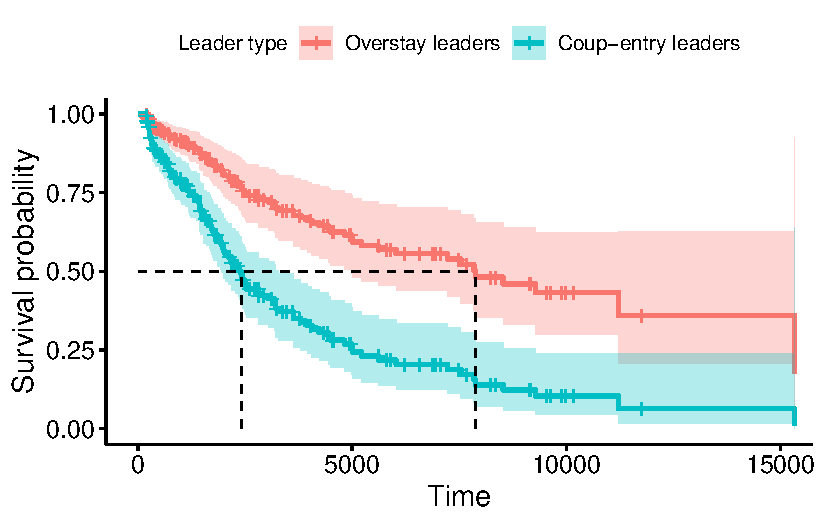
\includegraphics{survival_after_coups_jasa_files/figure-pdf/fig-coxSurv-1.pdf}

}

\subcaption{\label{fig-coxSurv-1}Cox PH Model}

\end{minipage}%
%
\begin{minipage}{0.50\linewidth}

\centering{

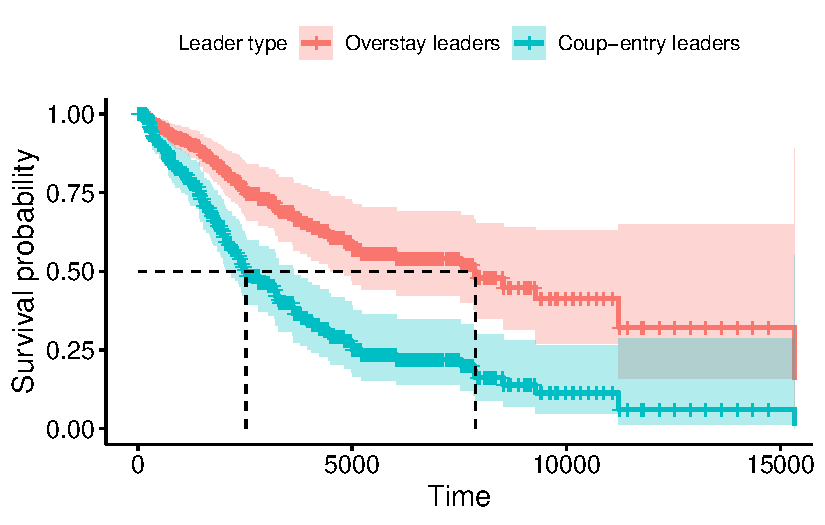
\includegraphics{survival_after_coups_jasa_files/figure-pdf/fig-coxSurv-2.pdf}

}

\subcaption{\label{fig-coxSurv-2}Time-dependent Cox Model}

\end{minipage}%

\caption{\label{fig-coxSurv}Survival curves for Cox Model}

\end{figure}%

The survival curves depicted in Figure~\ref{fig-coxSurv} illustrate the
respective survival rates for leaders of both types. Once more, both the
Cox proportional hazards (PH) model and the Time-dependent model
generate analogous plots. Notably, the survival curve for leaders who
enter through coups exhibits a significantly lower trajectory compared
to those who overstay their terms. This disparity suggests that
overstaying leaders are more inclined to endure for longer durations
than their coup-entry counterparts.

\begin{figure}

\begin{minipage}{0.50\linewidth}

\centering{

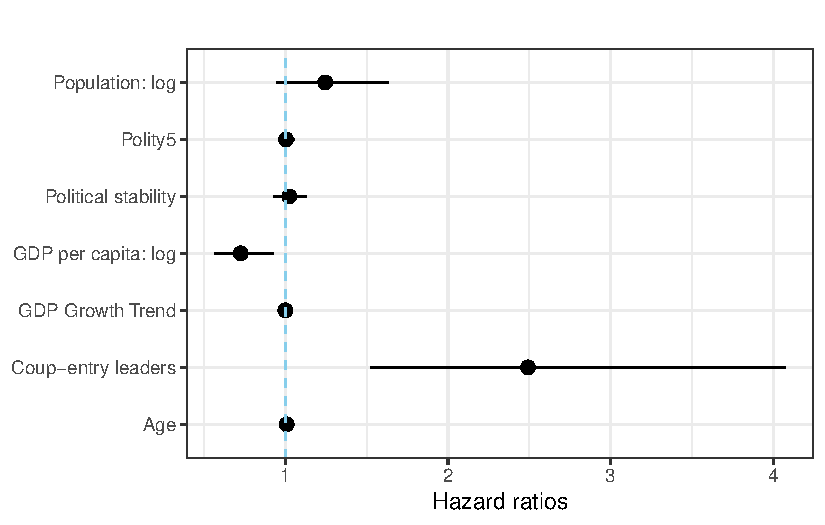
\includegraphics{survival_after_coups_jasa_files/figure-pdf/fig-coxHR-1.pdf}

}

\subcaption{\label{fig-coxHR-1}Cox PH Model}

\end{minipage}%
%
\begin{minipage}{0.50\linewidth}

\centering{

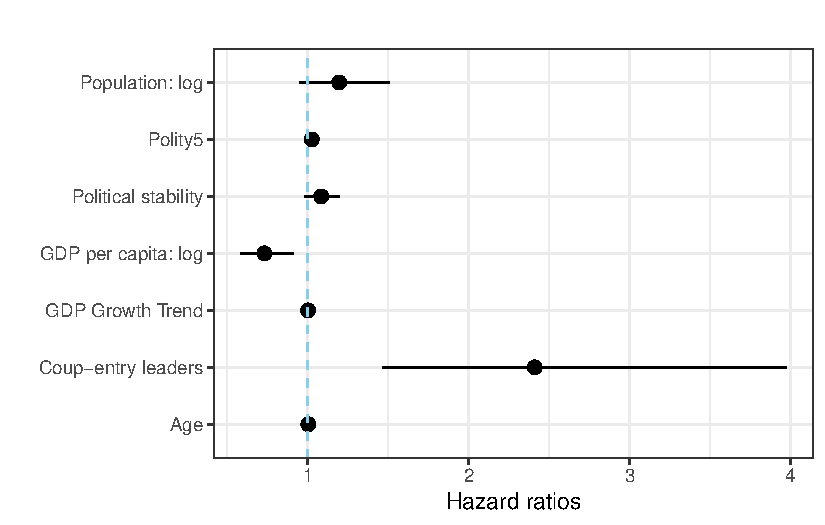
\includegraphics{survival_after_coups_jasa_files/figure-pdf/fig-coxHR-2.pdf}

}

\subcaption{\label{fig-coxHR-2}Time-dependent Cox Model}

\end{minipage}%

\caption{\label{fig-coxHR}Hazard ratios and 95\% CIs for Leader Ousting}

\end{figure}%

Figure~\ref{fig-coxHR} displays the hazard ratios and corresponding 95\%
confidence intervals for the variables incorporated in the Cox model.
Both the Cox proportional hazards (PH) model and the Time-dependent
model yield nearly identical plots. Notably, the hazard ratio for
leaders who assume power through coups and the logarithm of GDP per
capita emerge as statistically significant factors.

\newpage

\section{Conclusion}\label{conclusion}

\newpage


\renewcommand\refname{References}
  \bibliography{survival.bib}


\end{document}
